\section{Analysis 3: Do Frozen Models Benefit from Explicit Geometry?}

\paragraph{Motivation and hypotheses.} Idea 5 supplies explicit geometry (depth, segmentation, pose) for norm reasoning. Before training anything, we test two of its premises. \textbf{H1}: spatial content is concentrated in a subset of norm categories, which is where geometry should matter. \textbf{H2}: geometry maps give a frozen model usable information beyond the RGB frames they are derived from.

\paragraph{Data and protocol.} For H1 we count how often the correct answers of all 1{,}853 EgoNormia items \citep{rezaei2025egonormia} contain a term from a fixed spatial word list, by norm category. For H2, from the released 200-item verified split we keep one item per source video and take the 60 with the sharpest frames, a choice based on image quality alone. Six frozen models answer each item from (i) the answer options only, (ii) the options plus five pre-action RGB frames, and (iii) those plus estimated depth (Depth Anything V2) and instance segmentation (YOLOv8n-seg) of the same frames; as controls they also see the depth maps without RGB, the RGB grid three times, and another item's maps. Each answer is a separate call with no shared context and counts only if action and justification are both correct.

\begin{figure}[t]
\centering
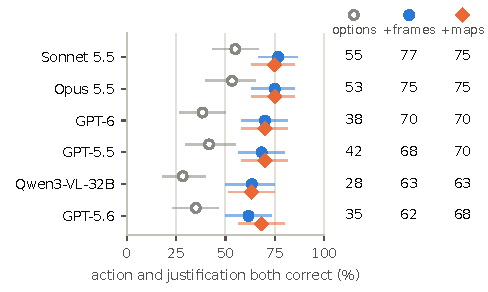
\includegraphics[width=\columnwidth]{analysis3_figure.pdf}
\caption{Joint accuracy of six frozen models on 60 items given the answer options only (grey), plus five RGB frames (blue), and plus depth and segmentation maps of those frames (orange). Lines are 95\% bootstrap intervals.}
\label{fig:a3}
\end{figure}

\paragraph{Results.} \emph{H1.} A spatial term appears in 24.6\% of correct answers, most often for Privacy (39.5\%) and Proxemics (33.4\%) and least for Cooperation (20.9\%): spatial content is concentrated, but it is a minority even in those categories. \emph{H2.} As a baseline, the options alone give 28--55\% and adding frames raises accuracy by 27 points on average (95\% interval [16, 38]; each model $p\le0.03$, exact McNemar), consistent with Analysis~1 (Figure~\ref{fig:a3}). A depth map without RGB adds 8 points over the options ([$-0.3$, 16]; five of six models improve), which suggests the maps carry some scene information. Added to the frames, however, depth and segmentation change accuracy by $-2$ to $+7$ points, $+1.1$ on average [$-1.7$, $+4.2$]: across 360 model--item pairs, maps correct 17 answers and break 13, and no model's change is significant; the largest is GPT-5.6's gain of four answers ($+7$ points, $p=0.12$). The 22 Proxemics items, where H1 says geometry should matter most, score 91 of 132 with or without maps. As a control, giving the same RGB grid three times instead of the maps does as well as the maps in all six models (256 vs.\ 253 of 360 answers correct; 249 with a single grid), and Qwen3-VL-32B scores 39/60 with another item's maps against 38 with its own.

\paragraph{Discussion of Analysis 3.} H1 holds in part and H2 does not. Spatial content concentrates in Proxemics and Privacy, but three in four correct answers use no spatial vocabulary, so geometry can matter only for a subset of the benchmark. The maps seem informative on their own, since depth without RGB tends to beat text, but they are redundant beside the frames: even on Proxemics items they neither help nor hurt, and repeating the frames does as well as adding them. Limits: 60 items detect only large effects (about $\pm12$ points per accuracy), a word list is a coarse measure of spatial content, and sharp verified frames are a best case for the extractors. Most importantly, this does not test Idea 5 itself: these models were presumably never trained to read depth or segmentation maps beside RGB, so a frozen model cannot be expected to use them. Fine-tuning a model on such inputs is the real test, and it is our next experiment.
